\documentclass[12pt,a4paper]{article}
\usepackage{amsmath,amscd,amsbsy,amssymb,latexsym,url,bm,amsthm}
\usepackage{epsfig,graphicx,subfigure}
\usepackage{enumitem,balance}
\usepackage{wrapfig}
\usepackage{mathrsfs,euscript}
\usepackage[usenames]{xcolor}
\usepackage{hyperref}
\usepackage[vlined,ruled,linesnumbered]{algorithm2e}
\usepackage{array}
\hypersetup{colorlinks=true,linkcolor=black}

\newtheorem{theorem}{Theorem}
\newtheorem{lemma}[theorem]{Lemma}
\newtheorem{proposition}[theorem]{Proposition}
\newtheorem{corollary}[theorem]{Corollary}
\newtheorem{exercise}{Exercise}
\newtheorem*{solution}{Solution}
\newtheorem{definition}{Definition}
\theoremstyle{definition}

\renewcommand{\thefootnote}{\fnsymbol{footnote}}

\newcommand{\postscript}[2]
 {\setlength{\epsfxsize}{#2\hsize}
  \centerline{\epsfbox{#1}}}

\renewcommand{\baselinestretch}{1.0}

\setlength{\oddsidemargin}{-0.365in}
\setlength{\evensidemargin}{-0.365in}
\setlength{\topmargin}{-0.3in}
\setlength{\headheight}{0in}
\setlength{\headsep}{0in}
\setlength{\textheight}{10.1in}
\setlength{\textwidth}{7in}
\makeatletter \renewenvironment{proof}[1][Proof] {\par\pushQED{\qed}\normalfont\topsep6\p@\@plus6\p@\relax\trivlist\item[\hskip\labelsep\bfseries#1\@addpunct{.}]\ignorespaces}{\popQED\endtrivlist\@endpefalse} \makeatother
\makeatletter
\renewenvironment{solution}[1][Solution] {\par\pushQED{\qed}\normalfont\topsep6\p@\@plus6\p@\relax\trivlist\item[\hskip\labelsep\bfseries#1\@addpunct{.}]\ignorespaces}{\popQED\endtrivlist\@endpefalse} \makeatother

\begin{document}
\noindent

%========================================================================
\noindent\framebox[\linewidth]{\shortstack[c]{
\Large{\textbf{Lab05-Linear Programming}}\vspace{1mm}\\
CS214-Algorithm and Complexity, Xiaofeng Gao, Spring 2019.}}
\begin{center}
\footnotesize{\color{red}$*$ If there is any problem, please contact TA Jiahao Fan.}

% Please write down your name, student id and email.
\footnotesize{\color{blue}$*$ Name: KylinChen  \quad Student ID: 517030910155 \quad Email: k1017856853@icloud.com}
\end{center}

\begin{enumerate}
    \item
    A company intends to invest $0.3$ million dollars in $2018$, with a proper combination of the following $3$ projects:
    \begin{itemize}
    \item \textbf{Project 1:} Invest at the beginning of a year, and can receive a $20\%$ profit of the investment in this project at the end of this year. Both the capital and profit can be invested at the beginning of next year;
    \item \textbf{Project 2:} Invest at the beginning of $2018$, and can receive a $50\%$ profit of the investment in this project at the end of $2019$. The investment in this project cannot exceed $0.15$ million dollars;
    \item \textbf{Project 3:} Invest at the beginning of $2019$, and can receive a $40\%$ profit of the investment in this project at the end of $2019$. The investment in this project cannot exceed $0.1$ million dollars.
    \end{itemize}
    Assume that the company will invest \emph{all} its money at the beginning of a year. Please design a scheme of investment in $2018$ and $2019$ which maximizes the overall sum of capital and profit at the end of $2019$.
    \begin{enumerate}
    \item
    Formulate a linear programming with necessary explanations.

    \item
    Transform your LP into its standard form and slack form.

    \item
    Transform your LP into its dual form.

    \item
    Use the simplex method to solve your LP by step.
    \end{enumerate}

    \begin{solution}\item
        \renewcommand{\qedsymbol}{}

        \begin{itemize}
        	\item [(a)] Assume that at the beginning of  2018, We invest $x_1$ (million dollars) in \textbf{Project 1}, $y$ in \textbf{Project 2}. While at the beginning of  2019, investing $x_2$ (million dollars) in \textbf{Project 1} and $z$ in \textbf{Project 3}.\\
        	In this case, we can give required constraint equations as follows:\\
          $$\text{max}\ f(x_1,y,z_1,x_2,z_2)=1.5y+1.2x_2+1.4z$$
          \textbf{s.t.}
          \begin{equation}
          x_1+y=0.3,
          \end{equation}
          \begin{equation}
          y \leq 0.15,
          \end{equation}
          \begin{equation}
          x_2+z = 1.2x_1,
          \end{equation}
          \begin{equation}
          z \leq 0.1,
          \end{equation}
          \begin{equation}
          x_1,y,x_2,z \geq 0.
          \end{equation}
          \textbf{Explaination:} Equation (1) and equation (3) means we will use all the money to invest at the beginning of every year. Equation (2),(4) and (5) is the original constrain.
        	\item [(b)] \textbf{Standard Form:}\\
        	$$\text{max}\ f(x_1,y,z_1,x_2,z_2)=1.5y+1.2x_2+1.4z$$
            \textbf{s.t.}
            $$x_1+y \leq 0.3,$$
            $$-x_1-y \leq -0.3,$$
            $$y \leq 0.15,$$
            $$x_2+z-1.2x_1 \leq 0,$$
            $$-x_2-z+1.2x_1 \leq 0,$$
            $$z \leq 0.1,$$
            $$x_1,y,x_2,z \geq 0.$$
          \textbf{Slack Form:}\\
          $$\text{max}\ f(x_1,y,z_1,x_2,z_2,m,n,p,q,w,s)=1.5y+1.2x_2+1.4z$$
            \textbf{s.t.}
            $$0.3-x_1-y = m,$$
            $$-0.3+x_1+y = n,$$
            $$0.15-y  = p,$$
            $$-x_2-z+1.2x_1=q,$$
            $$x_2+z-1.2x_1=w,$$
            $$0.1-z = s,$$
            $$x_1,y,x_2,z,m,n,p,q,w,s \geq 0.$$
        	\item [(c)] \textbf{Dual Form:}\\
        	Multiplier can refers to Table.1, So we can get dual form as follows:
        	$$\text{max}\ f(k_1,k_2,k_3,k_4,k_5,k_6)=0.3k_1-0.3k_2+0.15k_3+0.1k_6$$
            \textbf{s.t.}
            $$k_1-k_2+k_3 \leq 1.5,$$
            $$k_4-k_5 \leq 1.2,$$
            $$k_4-k_5+k_6 \leq 1.4,$$
            $$k_1,k_2,k_3,k_4,k_5,k_6 \geq 0.$$
            \begin{figure}[htbp]
            \centering
            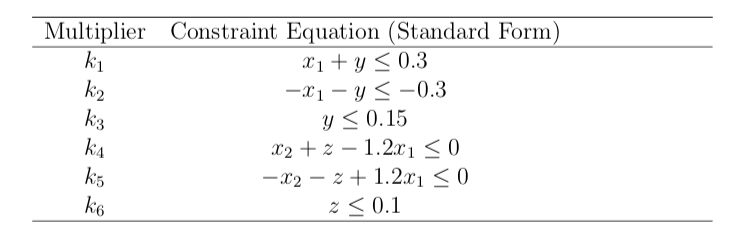
\includegraphics[width=0.8\textwidth]{figures/1_1.png}
            \caption{Dual form multiplier}\label{PNG1}
            \end{figure}\item
        	\item [(d)]\par
        	\textbf{Step 1:}\par
        	Base on the slack form:
        	$$\text{max}\ f(x_1,y,z_1,x_2,z_2,m,n,p,q,w,s)=1.5y+1.2x_2+1.4z$$
            \textbf{s.t.}
            $$0.3-x_1-y = m,$$
            $$-0.3+x_1+y = n,$$
            $$0.15-y  = p,$$
            $$-x_2-z+1.2x_1=q,$$
            $$x_2+z-1.2x_1=w,$$
            $$0.1-z = s,$$
            $$x_1,y,x_2,z,m,n,p,q,w,s \geq 0.$$
            Then we can get the basic solution:
            $$(x_1,y,x_2,z,m,n,p,q,w,s)=(0,0,0,0,0.3,-0.3,0.15,0,0,0.1)$$
            \textbf{Step 2:}\par
        	We can use the tightest constrain $-z+1.2x_1-q=x_2$ to replace $x_2$ to get a new basic solution as follows:
        	$$\text{max}\ f(x_1,y,z_1,x_2,z_2,m,n,p,q,w,s)=1.44x_1+1.5y+1.2(-q)+0.4z$$
            \textbf{s.t.}
            $$0.3-x_1-y = m,$$
            $$-0.3+x_1+y = n,$$
            $$0.15-y  = p,$$
            $$-z+1.2x_1-q=x_2,$$
            $$x_2+z-1.2x_1=w,$$
            $$0.1-z = s,$$
            $$x_1,y,x_2,z,m,n,p,q,w,s \geq 0.$$
            Then we can get the basic solution:
            $$(x_1,y,x_2,z,m,n,p,q,w,s)=(0,0,0,0,0.3,-0.3,0.15,0,0,0.1)$$
            \textbf{Step 3:}\par
        	We can use the tightest constrain $0.3-m-y = x_1$ to replace $x_1$ to get a new basic solution as follows:
        	$$\text{max}\ f(x_1,y,z_1,x_2,z_2,m,n,p,q,w,s)=1.44(0.3-m)+0.06y+1.2(-q)+0.4z$$
            \textbf{s.t.}
            $$0.3-m-y = x_1,$$
            $$-0.3+x_1+y = n,$$
            $$0.15-y  = p,$$
            $$-z+1.2x_1-q=x_2,$$
            $$x_2+z-1.2x_1=w,$$
            $$0.1-z = s,$$
            $$x_1,y,x_2,z,m,n,p,q,w,s \geq 0.$$
            Then we can get the basic solution:
            $$(x_1,y,x_2,z,m,n,p,q,w,s)=(0.3,0,0.36,0,0,0,0.15,0,-0.36,0.1)$$
            \textbf{Step 4:}\par
        	We can use the tightest constrain $0.15-p  = y$ to replace $y$ to get a new basic solution as follows:
        	$$\text{max}\ f(x_1,y,z_1,x_2,z_2,m,n,p,q,w,s)=1.44(0.3-m)+0.06(0.15-p)+1.2(-q)+0.4z$$
            \textbf{s.t.}
            $$0.3-m-y = x_1,$$
            $$-0.3+x_1+y = n,$$
            $$0.15-p  = y,$$
            $$-z+1.2x_1-q=x_2,$$
            $$x_2+z-1.2x_1=w,$$
            $$0.1-z = s,$$
            $$x_1,y,x_2,z,m,n,p,q,w,s \geq 0.$$
            Then we can get the basic solution:
            $$(x_1,y,x_2,z,m,n,p,q,w,s)=(0.15,0.15,0.18,0,0,0,0,0,0,0.1)$$
            \textbf{Step 4:}\par
        	We can use the tightest constrain $0.1-s = z$ to replace $z$ to get a new basic solution as follows:
        	$$\text{max}\ f(x_1,y,z_1,x_2,z_2,m,n,p,q,w,s)=1.44(0.3-m)+0.06(0.15-p)+1.2(-q)+0.4(0.1-s)$$
            \textbf{s.t.}
            $$0.3-m-y = x_1,$$
            $$-0.3+x_1+y = n,$$
            $$0.15-p  = y,$$
            $$-z+1.2x_1-q=x_2,$$
            $$x_2+z-1.2x_1=w,$$
            $$0.1-s = z,$$
            $$x_1,y,x_2,z,m,n,p,q,w,s \geq 0.$$
            Then we can get the basic solution:
            $$(x_1,y,x_2,z,m,n,p,q,w,s)=(0.15,0.15,0.08,0.1,0,0,0,0,0,0)$$
            \textbf{Conclusion:}Now we can find that the optimal solution for original problem is: 
            $$(x_1,y,x_2,z)=(0.15,0.15,0.08,0.1)$$ it means that, at the beginning of 2018, we invest \textbf{Project 1} 0.15 million dollars while \textbf{Project 2} 0.15 million dollars. At the end of 2018, we can get total 0.18 million dollars. Then at the beginning of 2019, we invest \textbf{Project 1} 0.08 million dollars while \textbf{Project 3} 0.1 million dollars.\\
            We can use the optimal solution to get the maximal profit $$f(x_1,y,z_1,x_2,z_2)=1.5y+1.2x_2+1.4z=1.5*0.15+1.2*0.08+1.4*0.1=0.461$$(scale: $million$ $dollars$).

        \end{itemize}
        
    \end{solution}

    \item
    An engineering factory makes seven products (PROD 1 to PROD 7) on the following machines: four grinders, two vertical drills, three horizontal drills, one borer and one planer. Each product yields a certain contribution to profit (in \pounds/unit). These quantities (in \pounds/unit) together with the unit production times (hours) required on each process are given below. A dash indicates that a product does not require a process.

    \begin{table}[htbp]
      \scriptsize
      \centering
      \renewcommand\arraystretch{1.1}
      \begin{tabular}{m{0.18\textwidth} m{0.07\textwidth}<{\centering} m{0.07\textwidth}<{\centering} m{0.07\textwidth}<{\centering} m{0.07\textwidth}<{\centering} m{0.07\textwidth}<{\centering} m{0.07\textwidth}<{\centering} m{0.07\textwidth}<{\centering}}
      \hline
       & \textbf{PROD 1} & \textbf{PROD 2} & \textbf{PROD 3} & \textbf{PROD 4} & \textbf{PROD 5} & \textbf{PROD 6} &  \textbf{PROD 7} \\\hline
      Contribution to profit & 10 & 6 & 8 & 4 & 11 & 9 & 3 \\
      Grinding & 0.5 & 0.7 & - & - & 0.3 & 0.2 & 0.5 \\
      Vertical drilling & 0.1 & 0.2 & - & 0.3 & - & 0.6 & - \\
      Horizontal drilling & 0.2 & - & 0.8 & - & - & - & 0.6 \\
      Boring & 0.05 & 0.03 & - & 0.07 & 0.1 & - & 0.08 \\
      Planing & - & - & 0.01 & - & 0.05 & - & 0.05 \\
      \hline
      \end{tabular}
    \end{table}

    There are marketing limitations on each product in each month, given in the following table:

    \begin{table}[htbp]
      \scriptsize
      \centering
      \renewcommand\arraystretch{1.1}
      \begin{tabular}{m{0.1\textwidth} m{0.07\textwidth}<{\centering} m{0.07\textwidth}<{\centering} m{0.07\textwidth}<{\centering} m{0.07\textwidth}<{\centering} m{0.07\textwidth}<{\centering} m{0.07\textwidth}<{\centering} m{0.07\textwidth}<{\centering}}
      \hline
       & \textbf{PROD 1} & \textbf{PROD 2} & \textbf{PROD 3} & \textbf{PROD 4} & \textbf{PROD 5} & \textbf{PROD 6} &  \textbf{PROD 7} \\\hline
      January & 500 & 1000 & 300 & 300 & 800 & 200 & 100 \\
      February & 600 & 500 & 200 & 0 & 400 & 300 & 150 \\
      March & 300 & 600 & 0 & 0 & 500 & 400 & 100 \\
      April & 200 & 300 & 400 & 500 & 200 & 0 & 100 \\
      May & 0 & 100 & 500 & 100 & 1000 & 300 & 0 \\
      June & 500 & 500 & 100 & 300 & 1100 & 500 & 60 \\
      \hline
      \end{tabular}
    \end{table}

    It is possible to store up to 100 of each product at a time at a cost of \pounds0.5 per unit per month (charged at the end of each month according to the amount held at that time). There are no stocks at present, but it is desired to have a stock of exactly 50 of each type of product at the end of June. The factory works six days a week with two shifts of 8h each day. It may be assumed that each month consists of only 24 working days. Each machine must be down for maintenance in one month of the six. No sequencing problems need to be considered.

    When and what should the factory make in order to maximize the total net profit?

    \begin{enumerate}
    \item
    Use \emph{CPLEX Optimization Studio} to solve this problem. Describe your model in \emph{Optimization Programming Language} (OPL). Remember to use a separate data file (.dat) rather than embedding the data into the model file (.mod).

    \item
    Solve your model and give the following results.
    \begin{enumerate}
    \item
    For each machine:
    \begin{enumerate}
    \item
    the month for maintenance.
    \end{enumerate}
    \item
    For each product:
    \begin{enumerate}
    \item
    The amount to make in each month.
    \item
    The amount to sell in each month.
    \item
    The amount to hold at the end of each month.
    \end{enumerate}
    \item
    The total selling profit.
    \item
    The total holding cost.
    \item
    The total net profit (selling profit minus holding cost).
    \end{enumerate}
    \end{enumerate}
    \begin{solution}\item
        \renewcommand{\qedsymbol}{}
        \begin{itemize}
          \item [(a)] \textbf{production.mod} and \textbf{production.dat} is attached in \textbf{.zip} file, which is tested in Mac OS X available.
          \item [(b)] We can use Cplex to get optimal solution, which can be give by follows:
          \begin{itemize}
            \item The following chart represent repairing month for all types of machines:
                \begin{figure}[htbp]
                \centering
                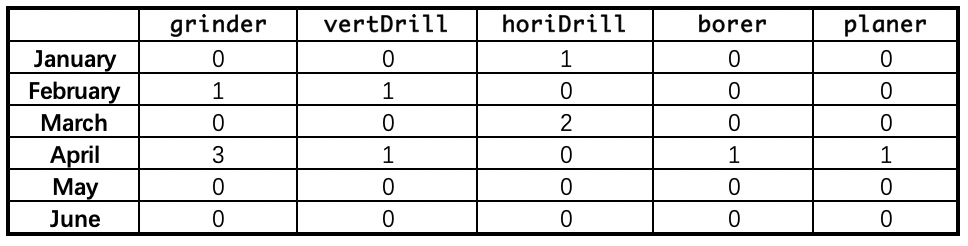
\includegraphics[width=0.8\textwidth]{figures/1_3.png}
                \caption{maintenance table}\label{PNG2}
                \end{figure}
            \item All arangement can be described by a chart attached in the last page:
                \begin{figure}[htbp]
                \centering
                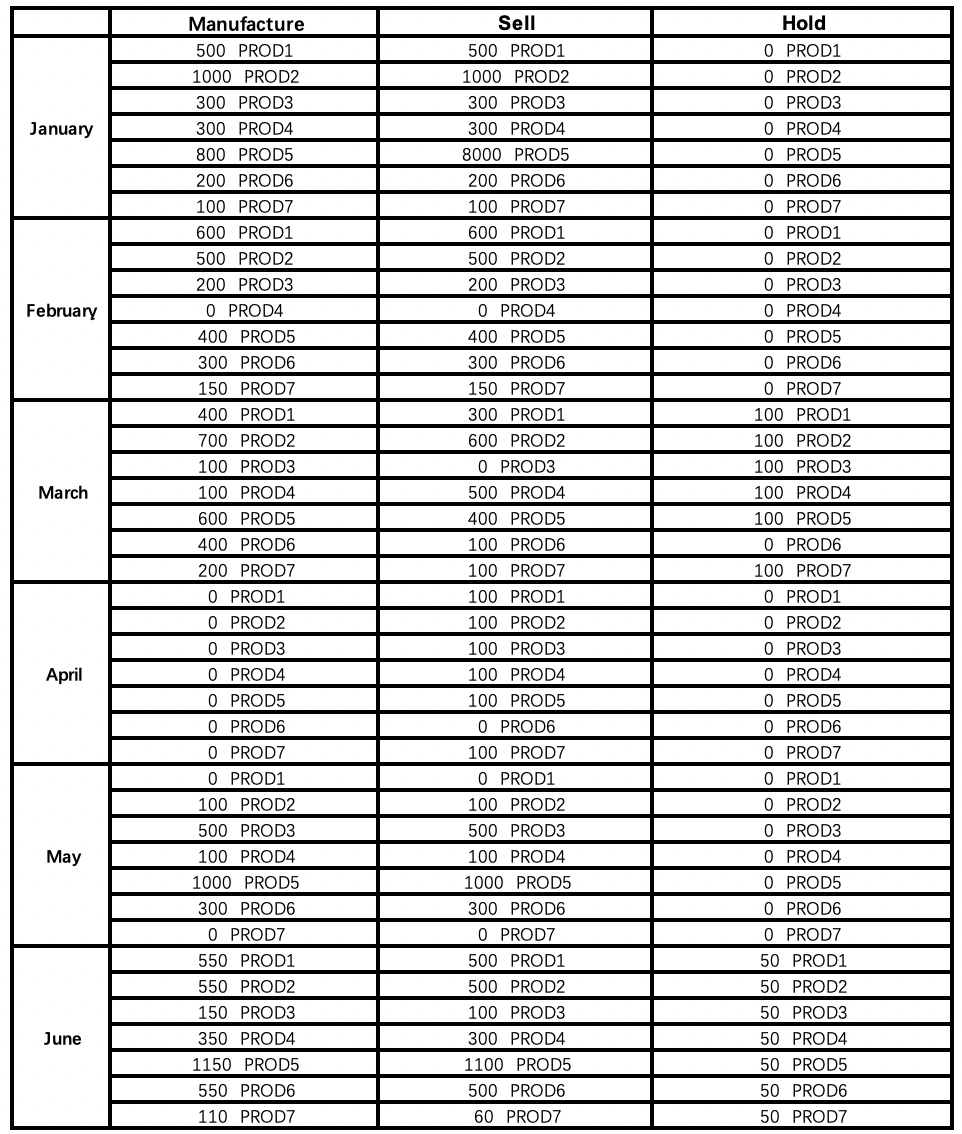
\includegraphics[width=0.9\textwidth]{figures/1_2.png}
                \caption{maintenance table}\label{PNG3}
                \end{figure}
            \item In Cplex solver, we can easily get this Three variables:\par
            \textbf{The total selling profit:} 109330 \pounds\par
            \textbf{The total holding cost:} 475 \pounds\par
            \textbf{The total net profit:} 108855 \pounds\par
          \end{itemize}
        \end{itemize}
    \end{solution}

\end{enumerate}

\vspace{20pt}


%========================================================================
\end{document}
